%%%% 1. DOCUMENTCLASS %%%%
\documentclass[journal=tosc,final]{iacrtrans}
%%%% NOTES:
% - Change "journal=tosc" to "journal=tches" if needed
% - Change "submission" to "final" for final version
% - Add "spthm" for LNCS-like theorems


%%%% 2. PACKAGES %%%tsdss
\usepackage[left, pagewise,edtable]{lineno}
\usepackage{blt}
\usepackage{graphicx}
\usepackage{framed} 
\usepackage{xcolor}
\usepackage{tcolorbox}
\usepackage{xcolor} 
\colorlet{shadecolor}{gray!25}
\definecolor{mshadecolor}{rgb}{0.7421875,0.7421875,0.7421875}
\setlength{\OuterFrameSep}{10pt}
%%%% 3. AUTHOR, INSTITUTE %%%
\author{Moritz Rupp}
\institute{
  Hochschule Albstadt-Sigmaringen, Albstadt, Germany, \email{ruppmori@hs-albsig.de}
  
}



%%%% 4. TITLE %%%%
\title{Sozio-Technische Lösungsansätze gegen Phishing}

\author{Moritz Rupp}

\begin{document}

\maketitle
\author


%%% 5. KEYWORDS %%%%s
\keywords{Social-Engineering \and Phishing \and IT-Security \and Container \and DNS }


%%%% 6. ABSTRACT %%%%s
\begin{abstract} Phishing zählt nach wie vor zu den häufigsten Methoden bei Cyberangriffen. Dabei werden versucht vertrauliche Informationen wie Passwörter oder Kreditkartennummern abzugreifen. Hierbei werden soziale Manipulationstechniken oder gefälschte Kommunikationskanäle genutzt, um das Vertrauen des Opfers zu gewinnen. Diese Arbeit untersucht Technische Lösungsansätze um dies vorzubeugen.  \end{abstract}

%%%% 7. PAPER CONTENT %%%%
\section{Einführung}
Phishing ist eine Form des betrügerischen Verhaltens im Internet, bei der Angreifer versuchen, sensible Informationen wie Benutzernamen, Passwörter, Kreditkartennummern oder andere persönliche Daten von Internetnutzern zu stehlen. Dies wird bewerkstelligt, indem Angreifer gefälschte Webseiten, E-Mails oder andere Kommunikationskanäle nutzen, um sich als vertrauenswürdige Quellen oder Organisationen auszugeben. Das Hauptziel des Phishings besteht immer darin, Opfer zu verleiten, ihre vertraulichen Informationen preiszugeben, indem sie beispielsweise auf einen gefälschten Link klicken, ihre Anmeldedaten auf einer gefälschten Website eingeben oder auf betrügerische E-Mails antworten.

Dazu nutzen Phishing-Angriffe oft soziale Manipulationstechniken, um das Vertrauen der Opfer zu gewinnen. Dies kann beispielsweise durch die Nachahmung von bekannten Unternehmen, Regierungsbehörden oder Finanzinstituten erfolgen. Die Angreifer verwenden entsprechende Sprache, gefälschte Logos und weitere Taktiken, um ihre gefälschten Kommunikationen authentisch wirken zu lassen.

Ein erfolgreicher Phishingangriff hat schwerwiegende Konsequenzen für die Opfer. Durch den Diebstahl persönlicher Daten können die Angreifer Identitätsdiebstahl begehen, finanziellen Schaden anrichten oder die gestohlenen Informationen für weitere kriminelle Aktivitäten nutzen. Darüber hinaus kann Phishing das Vertrauen der Benutzer in Online-Dienste und elektronische Kommunikation insgesamt untergraben.

Die Bekämpfung von Phishing erfordert eine Kombination aus technischen Lösungen, Benutzererziehung und rechtlichen Maßnahmen. Dies umfasst beispielsweise die Implementierung von Sicherheitsprotokollen wie E-Mail-Authentifizierung, Anti-Phishing-Filtern und Phishing-Warnungen in Webbrowsern. Die Sensibilisierung der Benutzer für Phishing-Techniken und die Förderung bewusster Online-Sicherheitspraktiken spielen ebenfalls eine wichtige Rolle bei der Verringerung des Risikos von Phishing-Angriffen.\\ Die Kombination von technischen und sozialen Komponenten und deren Abhängikeiten, kann als Sozio-technisches System bezeichnet werden. Die Strukturierung bzw. Beschreibung von solch einem System im Context von Phishing, kann hilfreich sein um die komplexe Landschaft aus Angriffvektoren und Präventivmaßnahmen richtig einordnen zu können. Diese Arbeit behandelt Sozio-technische Systeme  als Lösungsansatz gegen Phishing Angriffe. Dafür wird im ersten Schritt ein Sozio-technisches System definiert und auf Phishing angewand. Anschließend werden die teilkomponenten wie soziale und technische Lösungen vorgestellt und abschließend als gesamte Lösung zusammengeführt. 


\newpage
\section{Sozio-technisches System}
Ein Sozio-technisches System ist \dots.
\begin{center}
 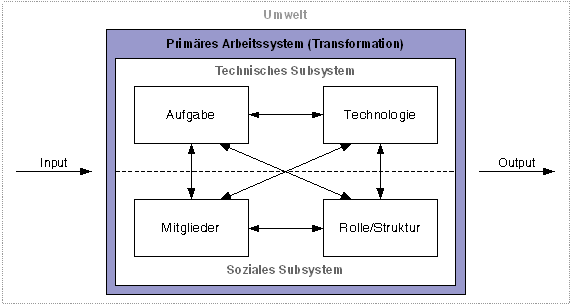
\includegraphics[scale=0.5]{sozio.png}

\end{center}
\dots
\section{Angriffslanndschaft}
\section{Systematik von Phishing Prävention}
\section{Technische Lösungsansätze}
\subsection{DNS-Header}
\section{Container}
\bibliographystyle{alpha}
\bibliography{ref.bib}
\end{document}
